\documentclass[12pt,letterpaper]{article}
\usepackage[utf8]{inputenc}
\usepackage[spanish]{babel}
\usepackage{graphicx}
\usepackage[left=2cm,right=2cm,top=2cm,bottom=2cm]{geometry}
\usepackage{graphicx} % figuras
% \usepackage{subfigure} % subfiguras
\usepackage{float} % para usar [H]
\usepackage{amsmath}
%\usepackage{txfonts}
\usepackage{stackrel} 
\usepackage{multirow}
\usepackage{enumerate} % enumerados
\renewcommand{\labelitemi}{$-$}
\renewcommand{\labelitemii}{$\cdot$}
% \author{}
% \title{Caratula}
\begin{document}

% Fancy Header and Footer
% \usepackage{fancyhdr}
% \pagestyle{fancy}
% \cfoot{}
% \rfoot{\thepage}
%

% \usepackage[hidelinks]{hyperref} % CREA HYPERVINCULOS EN INDICE

% \author{}
\title{Caratula}

\begin{titlepage}
\begin{center}
\large{UNERSIDAD PRIVADA DE TACNA}\\
\vspace*{-0.025in}
\begin{figure}[htb]
\begin{center}

\includegraphics[width=8cm]{./Imagenes/logo}
\end{center}
\end{figure}
\vspace*{0.15in}
INGENIERIA DE SISTEMAS  \\

\vspace*{0.5in}
\begin{large}
TITULO:\\
\end{large}

\vspace*{0.1in}
\begin{Large}
\textbf{TRABAJO DE INVESTIGACION  DE GITHUB} \\
\end{Large}

\vspace*{0.3in}
\begin{Large}
\textbf{CURSO:} \\
\end{Large}

\vspace*{0.1in}
\begin{large}
BASE DE DATOS II\\
\end{large}

\vspace*{0.3in}
\begin{Large}
\textbf{DOCENTE(ING):} \\
\end{Large}

\vspace*{0.1in}
\begin{large}
 Patrick Cuadros Quiroga\\
\end{large}

\vspace*{0.2in}
\vspace*{0.1in}
\begin{large}
Integrantes: \\
\begin{flushleft}
Coaquira Coaquira Guimer S.		\hfill	(2015053226) \\
\end{flushleft}
\end{large}
\end{center}

\end{titlepage}


\tableofcontents % INDICE
\thispagestyle{empty} % INDICE SIN NUMERO
\newpage
\setcounter{page}{1} % REINICIAR CONTADOR DE PAGINAS DESPUES DEL INDICE

\section{¿Que es GitHub?} 
GitHub es una plataforma de desarrollo colaborativo de software para alojar proyectos utilizando el sistema de control de versiones Git.
Nota:
El código se almacena de forma pública, aunque también se puede hacer de forma privada, creando una cuenta de pago.

\begin{center}

\includegraphics[width=14cm]{./Imagenes/imagen1} 
\end{center}

\section{¿Para que sirve?} 
GitHub aloja tu repositorio de código y te brinda herramientas muy útiles para el trabajo en equipo, dentro de un proyecto.
Además de eso, puedes contribuir a mejorar el software de los demás. Para poder alcanzar esta meta, GitHub provee de funcionalidades para hacer un fork y solicitar pulls.

\begin{center}

\includegraphics[width=14cm]{./Imagenes/imagen2} 
\end{center}
Además de eso, puedes contribuir a mejorar el software de los demás. Para poder alcanzar esta meta, GitHub provee de funcionalidades para hacer un fork y solicitar pulls.

\section{¿Qué herramientas proporciona?} 
En la actualidad, GitHub es mucho más que un servicio de alojamiento de código. Además de éste, se ofrecen varias herramientas útiles para el trabajo en equipo. Entre ellas, caben destacar:

\begin{center}

\includegraphics[width=14cm]{./Imagenes/imagen3} 
\end{center}

\begin{itemize}
\item Una wiki para el mantenimiento de las distintas versiones de las páginas.
\item Un sistema de seguimiento de problemas que permiten a los miembros de tu equipo detallar un problema con tu software o una sugerencia que deseen hacer.
\item Una herramienta de revisión de código, donde se pueden añadir anotaciones en cualquier punto de un fichero y debatir sobre determinados cambios realizados en un commit específico.
\item Un visor de ramas donde se pueden comparar los progresos realizados en las distintas ramas de nuestro repositorio.
\end{itemize}



\section{¿Qué uso le daremos?} 
En nuestra carrera de Ingenieria de Sistemas, fuimos aprendiendo cosas y creando aplicaciones en diferentes lenguajes, es por eso que presentamos esta gran herramienta enfocada al crecimiento de proyectos comunitarios y libres.

\begin{center}
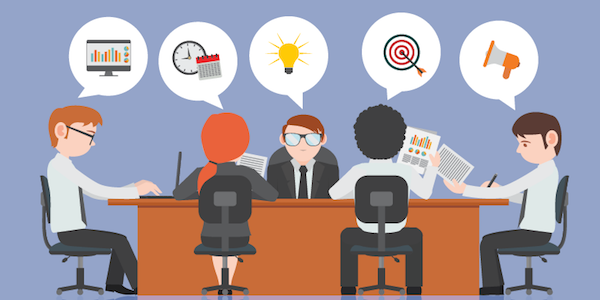
\includegraphics[width=14cm]{./Imagenes/imagen4} 
\end{center}

En esta página podremos crear una cuenta gratuita y comenzar a subir repositorios de código (o crearlos desde 0), para que con la ayuda de todos ese proyecto mejore; así como también fortalecer los proyectos de los demás para crecer como grupo.

\begin{center}
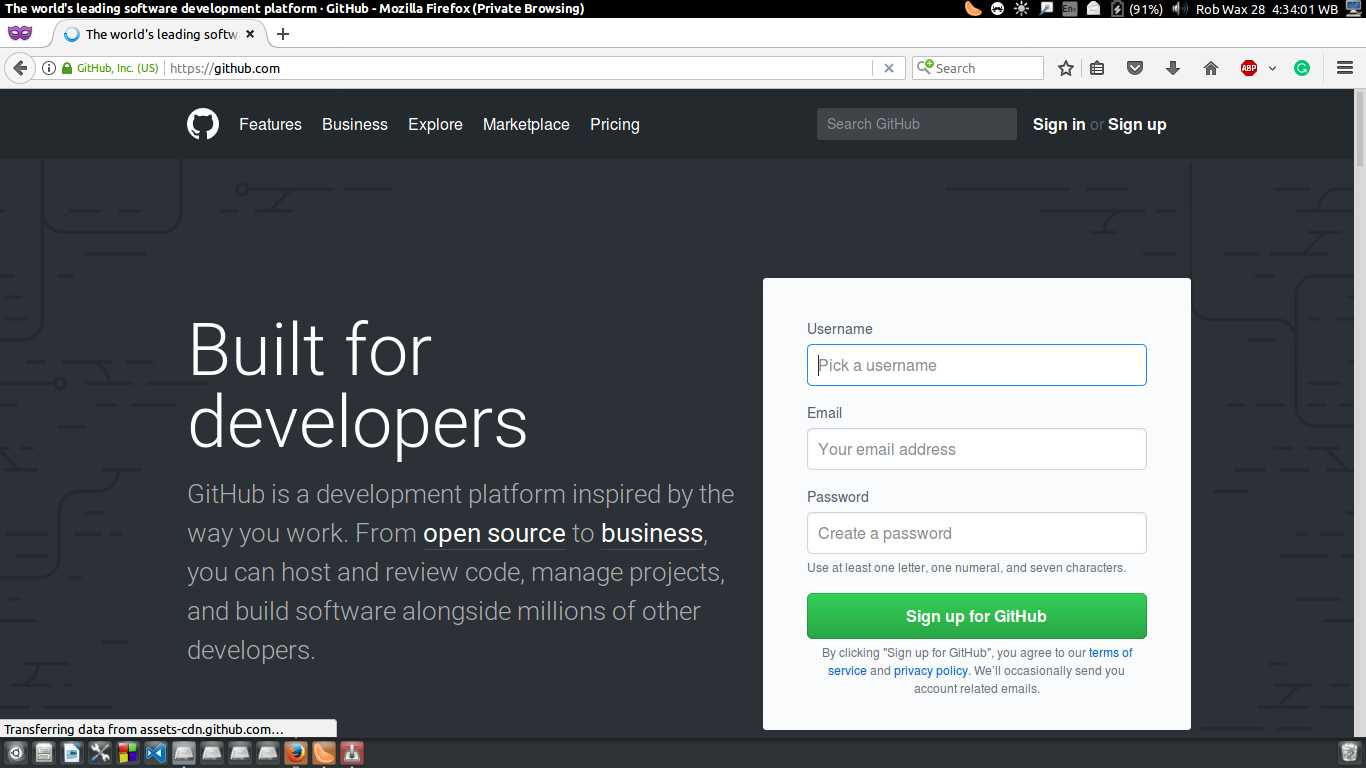
\includegraphics[width=14cm]{./Imagenes/imagen5} 
\end{center}

\section{CONCLUSIONES} 
\begin{itemize}
\item GitHub (y otras plataformas Web) son las nuevas herramientas en nuestra caja de herramientas de estudiantes.
\item Debemos analizarlas para comprender su papel e impacto.
\item Nuevos retos: integración, propiedad intelectual, nuevas herramientas de gestión...

\end{itemize}








\end{document}
